\documentclass[class=report,crop=false, 12pt]{standalone}
\usepackage[screen]{../scratch}

\begin{document}


\titre[E]{Créer ses blocs}
%===============================


\begin{enigme}

Je veux réaliser cette figure.
\begin{center}
  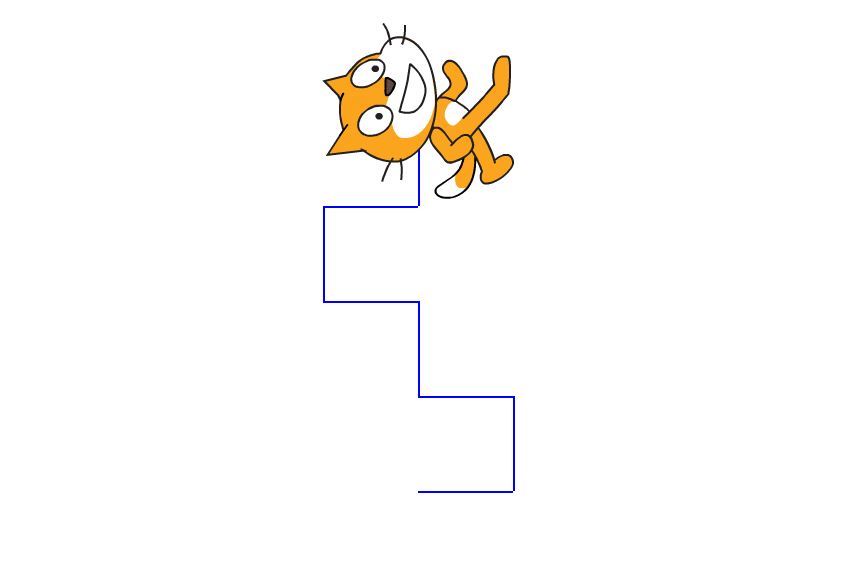
\includegraphics[scale=\scaleecran,scale=1.2]{ecran-11-eg1} 
\end{center}

\begin{minipage}{0.49\textwidth}
\begin{itemize}
  \item J'ai défini quatre nouveaux blocs : 
  \codeinline{monbloc1},  \codeinline{monbloc2},  \codeinline{monbloc3} et  \codeinline{monbloc4}.

\bigskip
  
  \item Lorsque le drapeau vert est cliqué, ces quatre blocs sont exécutés (une seule fois chacun).
  
\bigskip
  
  \item Malheureusement, j'ai oublié dans quel ordre je devais les placer afin de réaliser ma figure !
  
\end{itemize} 
\end{minipage}
\begin{minipage}{0.49\textwidth}
\begin{center}
  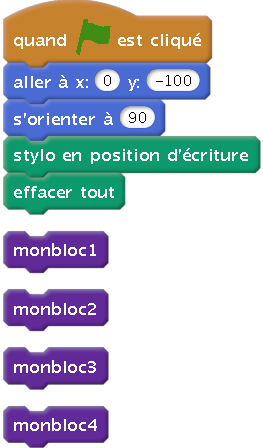
\includegraphics[scale=\scalebloc]{bloc-11-eg1a}
\end{center} 
\end{minipage}

Voici les quatre blocs que j'ai défini :
\begin{center}
  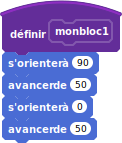
\includegraphics[scale=\scalebloc,scale=0.8]{bloc-11-eg1b}
  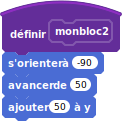
\includegraphics[scale=\scalebloc,scale=0.8]{bloc-11-eg1c}
  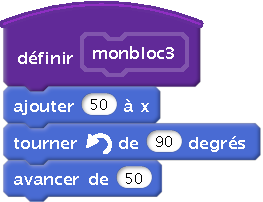
\includegraphics[scale=\scalebloc,scale=0.8]{bloc-11-eg1d}
  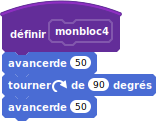
\includegraphics[scale=\scalebloc,scale=0.8]{bloc-11-eg1e}   
\end{center} 




\bigskip

\textbf{Question.} Quel doit être l'ordre des blocs ?


\emph{Répondre sous la forme d'un entier à quatre chiffres. Par exemple, s'il faut exécuter \codeinline{monbloc2}, puis
\codeinline{monbloc3}, puis \codeinline{monbloc1}, puis \codeinline{monbloc4}, alors répondre 2314.}

%\begin{solution}
%Réponse : 3241
%\end{solution}

\end{enigme}



\begin{enigme}

Je veux réaliser cette figure.
\begin{center}
  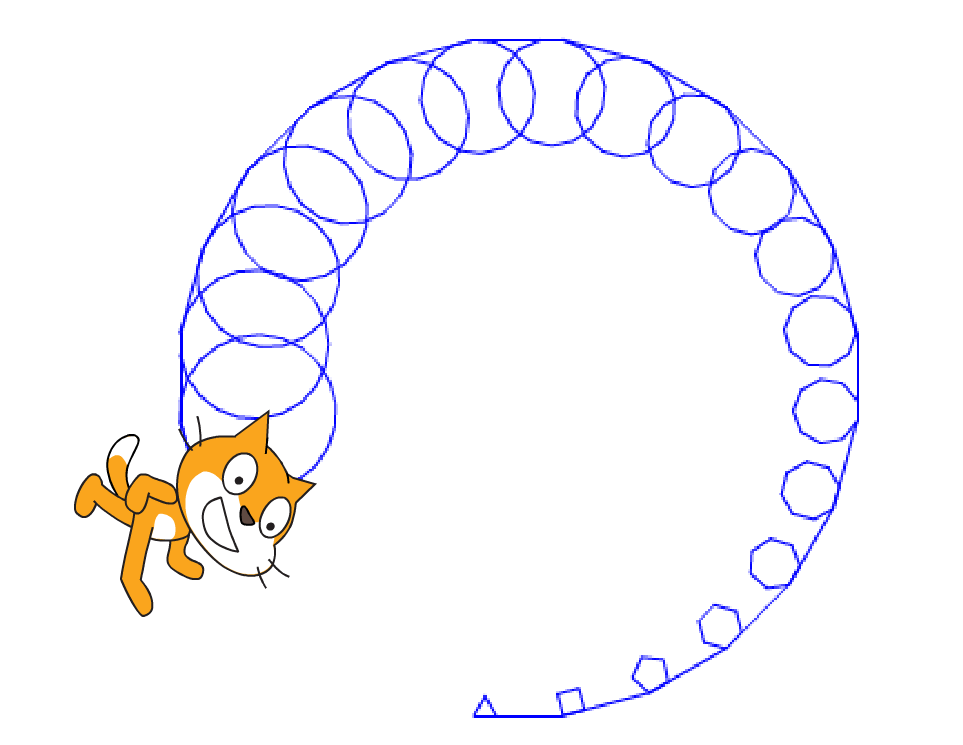
\includegraphics[scale=\scaleecran,scale=1.3]{ecran-11-eg2} 
\end{center}


\begin{minipage}{0.49\textwidth}
\begin{itemize}
  \item J'ai défini un nouveau bloc \codeinline{monbloc(n)} dont les instructions dépendent d'un entier $n$.

\bigskip
  
  \item Lorsque le drapeau vert est cliqué, la variable $n$ est initialisée à une certaine valeur, puis une boucle utilise plusieurs fois \codeinline{monbloc(n)}.
  
\bigskip
  
  \item Malheureusement, j'ai oublié à quelle valeur il faut initialiser la variable $n$ !
\end{itemize} 
\end{minipage}
\begin{minipage}{0.49\textwidth}
\begin{center}
  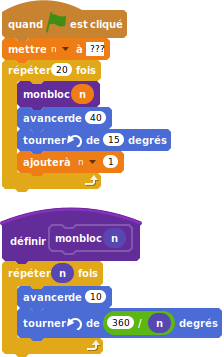
\includegraphics[scale=\scalebloc,scale=0.8]{code-11-eg2} 
\end{center} 
\end{minipage}


\bigskip

\textbf{Question.} Par quelle valeur faut-il remplacer les \og{}???\fg{} afin d'obtenir en fin d'exécution le dessin voulu ?

%\begin{solution}
%Réponse $n=3$ car \codeinline{monbloc(n)} dessine un polygone à $n$ côtés.
%\end{solution}

\end{enigme}


\begin{enigme}

Scratch doit dessiner cet arbre.
\begin{center}
  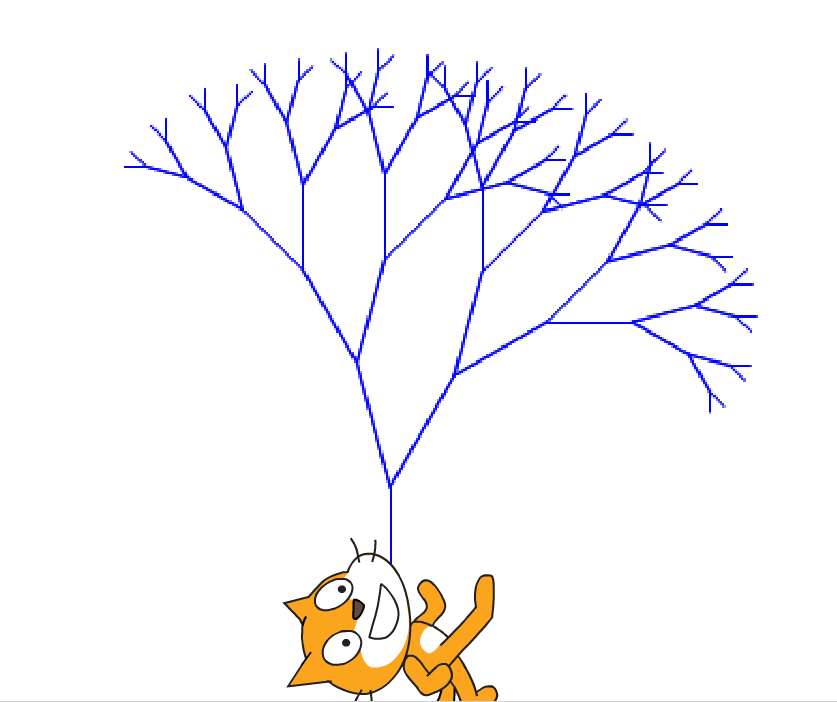
\includegraphics[scale=\scaleecran]{ecran-11-eg3} 
\end{center}


Voici le programme proposé !

\begin{center}
  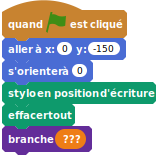
\includegraphics[scale=\scalebloc,scale=0.8]{bloc-11-eg3a}
  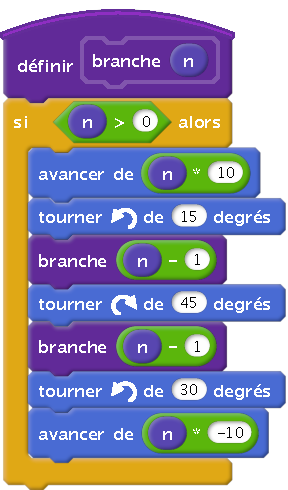
\includegraphics[scale=\scalebloc,scale=0.8]{bloc-11-eg3b}
\end{center} 
\begin{itemize}
  \item Il semble que le programmeur soit devenu fou, car dans l'écriture du bloc \codeinline{branche(n)}, le programme fait appel
au bloc \codeinline{branche} lui-même à travers l'instruction \codeinline{branche(n-1)}.

  \item Et pourtant cela fonctionne !
  
   \item Par contre, le programmeur a oublié de préciser la valeur (notée \og{}???\fg{} ci-dessus) avec laquelle est appelé le bloc \codeinline{branche} .
\end{itemize}


\bigskip

\textbf{Question.} Par quelle valeur faut-il remplacer les \og{}???\fg{} afin d'obtenir en fin d’exécution le dessin voulu ?


%\begin{solution}
%Réponse $n=7$.
%\end{solution}

\end{enigme}

\end{document}

